
\documentclass[11pt]{article}

% ************************ Font, typesetting **************************************

\usepackage[utf8x]{inputenc}
\usepackage{palatino}
\usepackage[bottom]{footmisc}
\usepackage{hyperref}

\usepackage{amsmath}


% for beautiful typesetting
\usepackage{microtype}

\usepackage{fancyhdr}
\usepackage{vmargin}
%  \setmarginsrb{leftmargin}{topmargin}{rightmargin}{bottommargin}
\setmarginsrb{2.5 cm}{1.5 cm}{2.5 cm}{1.5 cm}{1 cm}{1.5 cm}{1 cm}{1.5 cm}

% images
\usepackage{graphicx}

\usepackage{subcaption}
\usepackage{cleveref}
\captionsetup[subfigure]{subrefformat=simple,labelformat=simple}
\renewcommand\thesubfigure{(\alph{subfigure})}

\usepackage{float}
\usepackage{enumitem}

\newenvironment{longdescription}
  {\begin{description}[style=unboxed]}
  {\end{description}}

% ************************ Coloring *******************************************
\usepackage{xcolor}

\definecolor{black}{rgb}{0.0, 0.0, 0.0}

\hypersetup{
    colorlinks,
    linkcolor={black},
    citecolor={black},
    urlcolor={black}
}

% ************************ Header/footer ***************************************

%\setlength{\headheight}{2cm}
\pagestyle{fancy}
\fancyhf{}
\rhead{TILES Feasibility Study}

\cfoot{\thepage}
\rfoot{\href{https://www.pngk.org/}{
\includegraphics[width=1.25cm]{images/PNGK_logo.png}}}


\newcommand{\appendixpagenumbering}{
  \break
  \pagenumbering{arabic}
  \renewcommand{\thepage}{\thesection-\arabic{page}}
}

%  Appendix
\usepackage[toc,page]{appendix}




% Side by side images
\newcommand*{\twoImages}[8]{
	\begin{figure}[H]
		\centering
		  \begin{subfigure}{0.475\textwidth}
			\includegraphics[width=\textwidth, scale=0.5]{#1}
			  \caption{#2}
			  \label{#3}
		  \end{subfigure}
		  \hfill
		  \begin{subfigure}{0.475\textwidth}
			\includegraphics[width=\textwidth, scale=0.5]{#4}
			  \caption{#5}
			  \label{#6}
		  \end{subfigure}
	\caption{#7}
	\label{#8}
	\end{figure}
}

\begin{document}

\begin{titlepage}
\centering

    % title
	\textsc{\textbf{\huge{TILES Feasibility Study}}} \\[0.25 cm]
	\textsc{\huge{Borno State, Nigeria }}\\[0.25 cm]
	\vspace*{1\baselineskip}
	
	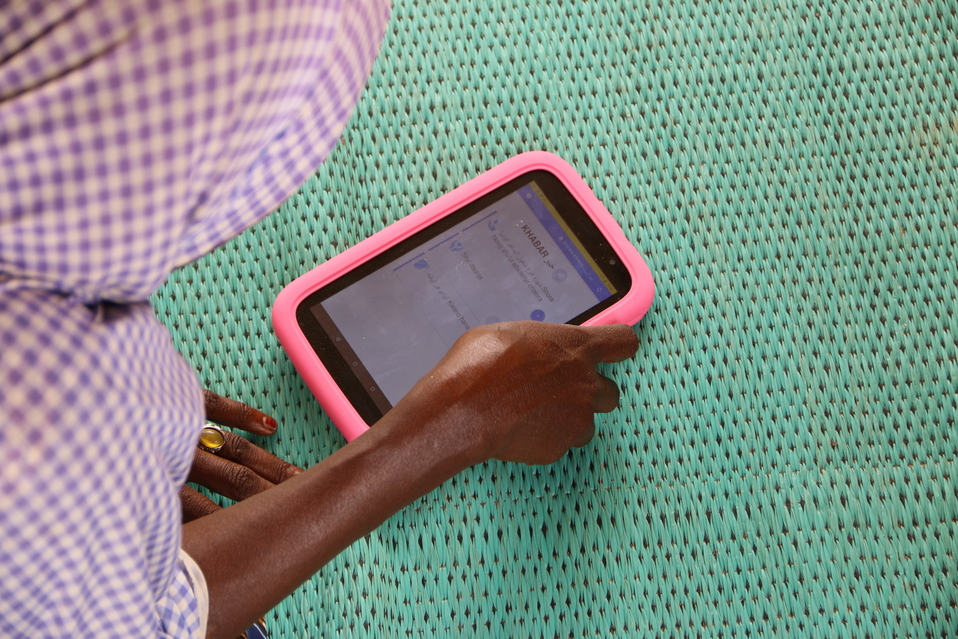
\includegraphics[width=16cm, scale=0.25]{images/woman_using_TILES.JPG} \\[1cm]

	\Large{A report summarizing observations made during November 18th to December 1st 2019, where six IDP camps were visited and user testing was performed.} \\[2 cm]
	

	\href{https://www.pngk.org/}{\textsc{
\includegraphics[width=3cm]{images/PNGK_logo.png}}} \\[0.15cm]
	

	% authors
	\noindent
    \begin{minipage}[b]{.5\textwidth}
        \centering
        \href{mailto:eric@pngk.org}{eric@pngk.org}
    \end{minipage}%
	\\[2.5cm]
	
	\today

\end{titlepage}

% ==============================================================================
\section*{Summary}
% ==============================================================================
From November 18th 2019 - December 1st 2019 Eric from PNGK visited the TWB Nigeria team in Maiduguru. During this trip six IDP camps were visited, three around Maiduguru and three in Gwoza, camp staff were interviewed and TILES was tested. For the visit it was collectively decided to concentrate on the information dissemination features of TILES. Therefore the TILES feedback mechanism was not tested. The main takeaways from this visit are:
\begin{itemize}
	\item There was an interest in the app from all groups we showed the app to, groups being:
		\begin{itemize}
			\item Residents of the IDP camps
			\item Management of the IDP camps
			\item NGO staff
		\end{itemize}
	\item Residents of the IDP camps mostly utilized the audio feature of the app, even the literate ones.
	\item The younger members of TWB’s staff (e.g. Shettima and Ibrahim) are eager and capable of working with TILES content format, Markdown, confirming TWB will be able to add content to TILES.
	\item The author estimates that 25\% of the camp residents who tried TILES asked if/how they could speak into it. Meaning they wanted to use it to provide feedback.
\end{itemize}

% ==============================================================================
\section{Observations of IDP Camps in Borno State}
% ==============================================================================

All of the camps we visited in Borno State had a permanent feel like they had been there for a while. 

\twoImages{images/gubio_camp_tents.JPG}
{Gubio camp outside Maiduguru}
{}
{images/GSS_camp_tents.jpg}
{GSS camp in Gwoza}
{}
{Camps having a permanent look and feel}
{}

Further information about the six camps visited can be found in Appendix~\ref{appendix:A} or in \textit{\href{https://docs.google.com/spreadsheets/d/1rCOyarp6DPsEXrMNfqc4tc5QZQE-FpaC5VYvPes1D0E/edit?usp=sharing}{this google sheet}}. 

\subsection{Security / camp access}

The camps could be broken into two categories in terms of security and accessability. 

\begin{description}[style=unboxed,leftmargin=0cm]

	\item [\textsc{Fenced camps}] These camps are surrounded by a fence and have a main gate with a security checkpoint where you need to sign in and sign out.  All of three of the camps we visited in Maiduguru were fenced camps. 
	
	\twoImages{images/Fenced_idp_helecopter.png}
	{IDP camp outside Maiduguru}
	{fig:fenced_helecopter}
	{images/teachers_village_gate.png}
	{Gate to Teachers Village Camp}
	{fig:fenced_gate}
	{Examples of fenced camps}
	{}

	\item [\textsc{Open camps}] These camps have no fence or official security checkpoint, people move freely in and out of them. All of the camps in Gwoza would fall under this category. 
	
	\twoImages{images/GSS_camp_helecopter.png}
	{GSS Camp in Gwoza}
	{fig:open_helecopter}
	{images/GSS_camp_people_leaving.png}
	{People leaving GSS}
	{fig:open_gate}
	{Examples open camps}
	{}

\end{description}

\subsection{Main office in the camp}

All of the camps had a main office near the entrance. For example Figure~\ref{fig:teachers_view} showcases the layout of Teachers Village Camp where the blue arrow points to the camp office and the yellow arrow points to the camp entrance, which is also shown in Figure~\ref{fig:fenced_gate}. 

All of the camps we visited were managed by IOM, therefore we would always start our visit by meeting with IOM camp managers. In the Gwoza camps we also met with community leaders. The camp offices were always quite busy as they appeared to be an assembly point for people to meet. 

\begin{figure}[H]
	\centering
	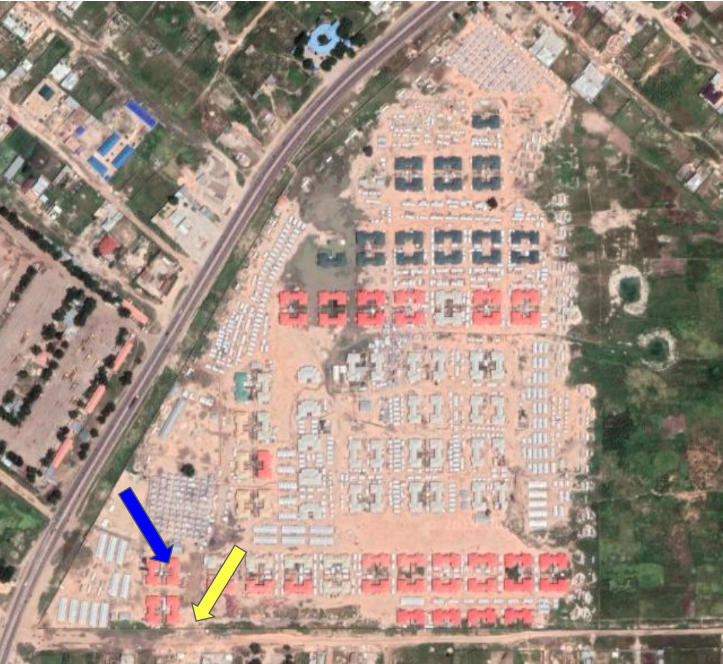
\includegraphics[width=0.6\textwidth, scale=0.5]{images/teachers_village_above.png}
	\caption{Teachers Village Camp. Blue arrow shows the camp office and the yellow arrow shows the main gate}
	\label{fig:teachers_view}
\end{figure}

None of the camp offices visited had electricity. The ones visited could be classified into two categories.

\begin{description}[style=unboxed,leftmargin=0cm]

	\item [\textsc{Permanent Office}] A permanent office is one which has a permanent structure e.g. mason building with steel doors. Four of the six camps we visited fell under this category, all of these offices had a secure room which the camp managers said could most likely be (approval of IOM supervisor would be required) used for storage of TILES tablets and other electronics. 
	
	\twoImages{images/GSS_camp_office_inside.jpg}
	{Inside the GSS camp office in Gwoza}
	{}
	{images/bakassi_camp_office.jpg}
	{Entrance to the Bakassi camp office in Maiduguru}
	{}
	{Examples of permanent offices}
	{}

	\item [\textsc{Temporary Office}] Temporary offices are ones made out of temporary structural materials such as a light timber frame, plastic sheeting and a thin metal roof. These offices would not be secure enough to store the tablets.
	
	\twoImages{images/wakane_camp_office.jpg}
	{Wanake camp office in Gwoza}
	{}
	{images/wakane_camp_office_inside.png}
	{Inside the Wakane camp office}
	{}
	{Examples temporary offices}
	{}

\end{description}

\subsection{Camp Zones and Zone Leaders}
All of the camps are broken down in a similar manner. They have what some people refer to as Zones and Zone leaders. A zone represents a physical area in a camp and the zone leader is the community representative of a specific zone. 

It was almost universally suggested that, if we decided to bring tablets to the camp, the zone leaders should be responsible for collecting one or two tablets each morning. Bringing them to their zone, showing people how to access information on TILES and then returning the TILES tablet to the camp office at the end of the day. 

Based on the authors experience showing people how to use TILES there seems to be no reason why these zone leaders could not be trained on how to use TILES and therefore help people in their zone access information through TILES. 

\subsection{Internet access}
The three camps in or around Maiduguri all had access to a 4G GSM network. The internet was observed to be strong and fast enough to allow for TILES to be downloaded and updated when paired with. All of Gwoza had no GSM network and multiple cell towers in Gwoza were visibly damaged. 

\twoImages{images/gwoza_down_gsm_tower.png}
{A partially built and a damaged GSM tower}
{}
{images/gwoza_down_gsm_tower_hele.png}
{Another damaged GSM tower}
{}
{Gwoza destruction of GSM towers}
{}

In Gwoza there is satellite internet connection at the Humanity Hub compound, that should be strong enough to enable the TILES app to be download and updated. 

% ****************************************************************
%                      User Testing
% ****************************************************************
\section{User testing}

In all of the camps we asked the people whom we met with to try the TILES device. In four of the camps we walked around, approached random people in the camp, asked them to use the TILES device and we gathered feedback.

\subsection{Meeting with camp residents}

\textit{"He was excited to hear Waha on the device and said he never thought his language might be considered so important to be put on a device."}

\twoImages{images/user_testing/woman_with_TILES.JPG}
{Woman using TILES}
{}
{images/user_testing/man_with_TILES.JPG}
{Man using TILES}
{}
{People using TILES at Gubio Camp in Maiduguru}
{}

We spoke with women and men, young and old, everyone positively viewed TILES and when asked said they would want it at their camps. 

People who have experience with smartphones were able to utilize TILES with no assistance. The functionality and buttons were all obvious to them. Adults who had little or no experience with smartphones before were more hesitant to use TILES and had to be shown how to do so. All of the children who used TILES were able to figure it out with no or little help.

The audio feature of the app was the most commonly used feature, even the literate people chose to listen to the audio over reading the text. The speakers on the Tablets are not strong enough to allow for a group to listen to TILES. One or two people were able to listen to TILES information at a time. 

\twoImages{images/user_testing/group_with_tiles.jpg}
{TILES demo at Teachers Camp}
{}
{images/user_testing/kid_sun_using_TILES.png}
{A kid who learned how to use TILES with minimum help}
{}
{Groups around TILES demonstrations}
{}
\subsection{TILES user interface design}

An iterative design process was done with the TILES user interface during the two week trip. Figure \ref{fig:start_tiles_ui} shows the user interface design that was brought to Maiduguru and Figure \ref{fig:final_tiles_ui} shows us the user interface at the end of the user testing visit. 

The user interface changes which were made, and the reasons why are listed below.

\begin{description}[style=unboxed,leftmargin=0cm]

	\item [\textsc{Each language has its own primary and secondary color.}] TWB staff in the Red Roof Maiduguru office said that every languages had common colors. Using these colors would make it easier for people to distinguish their language.
	
	\item [\textsc{Each language has a unique image.}] The TWB staff said these images would help people identify their language, this was confirmed during user field testing.
	
	\item [\textsc{A button sideways triangle was used to represent play audio.}] This icon was recommended from multiple people living in the refugee camps, once it was implemented people - who had used devices before - were able to recognize it as button which would play something. 
	
	\item [\textsc{Buttons are big and the same color.}] When the the play button and next page buttons were different colors they seemed to confuse people. Once the buttons were made the same color for each language and their size was increased, people appeared to be able to use TILES more efficiently. At least we did not receive any more comments about the buttons being an issue.  
	
	\item [\textsc{Large back button on the top left.}] Some people did not know how to use the android back button so this button helped them.

	\item [\textsc{On the language select page the buttons bounce when a user presses something other than the buttons}] People would try and click a photo expecting that to do something. We introduced a feature that caused the buttons to bounce when a user clicked something other than the button. This drew the user's attention to the buttons which would cause the user to click them. 


\end{description}


\twoImages{images/user_testing/TILES_old_language_select.png}
{Language select screen}
{}
{images/user_testing/TILES_old_welcome_page.png}
{Welcome screen}
{}
{TILES at the start of visit to Maiduguru}
{fig:start_tiles_ui}

\twoImages{images/user_testing/TILES_final.png}
{Language select screen}
{}
{images/user_testing/TILES_final_welcome.png}
{Welcome screen}
{}
{TILES user interface after iterations}
{fig:final_tiles_ui}


\subsection{Smartphones in the camps}
There is no data which can be used to estimate the number of smartphones in the camp. We asked camp managers to estimate the percentage of households who had smartphones and it was between 1\% and 10\% depending on the camp. 

Figure \ref{fig:mans_own_phone} shows a man at Teachers Village who was able to install and access the TILES app on his smartphone. He accessed the internet via the authors iphone7 hotspot on the MTN Network. Another man was able to use TILES on his phone but only after updating Google Chrome. 

A noteworthy event happened when visiting Teachers Village Camp, when Amajam from TWB asked at the same time 7 teenage girls if they had a smart phone. Three of the seven had a smart phone with them. One of the girls had the smart phone shown in Figure \ref{fig:inifix} which the author observed multiple people having in the camp. The author attempted to download TILES on this phone however it appeared that Google Chrome needed to be updated and during the update the internet credit expired. This shows that in order for people to use TILES on their personnel devices they also may need to update Google Chrome on their personnel devices. 

\twoImages{images/user_testing/smart_phone_tiles.png}
{Camp resident downloaded TILES on their phone}
{fig:mans_own_phone}
{images/user_testing/typical_phone.png}
{Infinix Hot smartphone}
{fig:inifix}
{TILES user interface after iterations}
{fig:final_tiles_ui}

\newpage
\section{Suggested functionality of the admin interface}

The admin interface is what TWB staff will need to use in order to add and remove content from TILES. It is clear that some of TWB's staff will be able to use the Markdown markup format for creating the content.

The features recommended for the admin interface are:

\begin{description}[style=unboxed,leftmargin=0cm]

	\item [\textsc{User profiles}] Each TWB staff member should have their own profile when they the TILES admin interface.
	
	\item [\textsc{Markdown rendering}] The TILES admin interface at a minimum should be able to render all markdown files so they can be visually checked. 
	
	\item [\textsc{Offline capable}] While the TWB office at the Red Roof compound has internet it can be slow and during the visit the internet network was observed to be not functioning for over a minute 1-10 times daily. It would be helpful if the admin interface could work offline. 
	
	\item [\textsc{Save entries to work on later}] TWB staff should be able to save the entries they are working on so they can come back and work on them before publishing.  
	
	\item [\textsc{Audio playback}] Users should be able to play back the audio files they have uploaded to ensure they are the correct one and that the quality is satisfactory.

\end{description}

\section{Questions for TWB to consider}
The following questions were raised during the visit which could be useful to answer as the project moves into its second phase. 

\begin{itemize}
	\item How will the tablets be charged and updated?
	\item Is there a scenario where it is desired to allow people to be able to access TILES from their own devices? E.g. Figure \ref{fig:mans_own_phone}.
	\item People were very excited about TILES however, is this because it was a fancy new app or that it is something they will use in the long term?
	\item Will there be enough content to keep people interested enough to regularly visit TILES?
	\item What will the content generating workflow look like, who will the content come from?
	\item Are the personnel and facilities available to make all of the required audio content?
	\item Should the devices be modified to make them more audible in the camps? If so what will that modification look like?
	\item What will the technical party's role look like during the second phase of TILES?
	\item What would you define as a successful second phase of TILES?
\end{itemize}

\newpage

\begin{appendices}
  \section{Camp features table}\label{appendix:A}
  
	\begin{table}[h]
    \centering
\small
  \begin{tabular}{|p{2cm}|p{2cm}|p{2cm}|p{1.75cm}|p{1.75cm}|p{1.75cm}|p{2cm}|}
\hline
    \textbf{Camp Name} & \textbf{Location (city)} & \textbf{Location (Lat Long)} & \textbf{GSM Network} & \textbf{Camp office} & \textbf{Security} & \textbf{Number of Households} \\ \hline
    Giubio Camp & Maiduguri & 11°54'12.3"N 13°04'47.2"E & Yes & Permanent Office & Fenced camp & 6013 \\ \hline
    Bakassi Camp & Maiduguri & 11°47'27.8"N 13°07'13.6"E & Yes & Permanent Office & Fenced camp & 7320 \\ \hline
    Teachers Village Camp & Maiduguri & 11°50'33.2"N 13°05'57.0"E & Yes & Permanent Office & Fenced camp & 6911 \\ \hline
    Wakane & Gwoza & 11 5' 22" N 13 41' 17"E & No & Temporary Office & Open camp & 199 \\ \hline
    20 Housing Camp & Gwoza & 11°04'14.8"N 13°41'26.2"E & No & Temporary Office & Open camp & 784 \\ \hline
    GSS Camp & Gwoza & 11°06'21.0"N 13°41'30.0"E & No & Permanent Office & Open camp & 1273 \\ \hline
    
    \end{tabular}
    \end{table}
     
\end{appendices}


\end{document}


